% Work-MAT -- 2. rocnik, hodina 03. Inverze vyhradne graficky.
\documentclass[11pt,a4paper]{article}
\input{../../sablony/pripravy/priprava.sty}
\usepackage{tikz}
\usetikzlibrary{arrows.meta}
\nastavPripravu{2. ročník}{Inverzní funkce}{03}{Inverzní funkce I: graficky}
\begin{document}
\poznamka{Nová látka začíná graficky. Navazuj na myšlenkovou mapu z hodiny 02: vztah mezi argumentem a funkční hodnotou. V této hodině nepočítej předpis inverzní funkce; veškeré závěry odvozuj z grafu, bodů a osové souměrnosti podle $y=x$.}

\blok{Prostota: kdy lze přiřazení obrátit?}
Na grafu funkce $f$ odpovídá každému argumentu $x$ právě jedna funkční hodnota $y$. Chceme-li postup obrátit, musí každé funkční hodnotě odpovídat právě jeden původní argument. To nemusí být splněno: například u paraboly $y=x^2$ mají argumenty $-2$ a $2$ stejný obraz $4$.

\begin{definiceBox}[title={Definice - Prostá funkce}]
Funkce $f$ je \textbf{prostá}, jestliže různým argumentům přiřazuje různé funkční hodnoty. Formálně pro všechna $x_1,x_2\in D(f)$ platí
\[
f(x_1)=f(x_2)\ \Longrightarrow\ x_1=x_2.
\]
\end{definiceBox}

\begin{prikladReseniBox}[title={Příklad 1}]
Graficky rozhodni, která z funkcí $f(x)=x+1$ a $g(x)=x^2$ na $\mathbb R$ je prostá. Použij vodorovnou přímku.
\tcblower
Graf přímky $y=x+1$ protne každá vodorovná přímka nejvýše jednou; funkce $f$ je prostá. U paraboly $y=x^2$ může vodorovná přímka protnout graf ve dvou bodech, například v $[-2;4]$ a $[2;4]$. Funkce $g$ proto na $\mathbb R$ prostá není.
\end{prikladReseniBox}

\begin{center}
\begin{minipage}{.45\linewidth}\centering
\begin{tikzpicture}[x=.62cm,y=.62cm,>=Latex]
\draw[->](-2.8,0)--(2.9,0)node[right]{$x$};
\draw[->](0,-2.5)--(0,3.2)node[above]{$y$};
\draw[very thick](-2.5,-1.5)--(1.8,2.8);
\draw[densely dashed](-2.6,1.5)--(2.7,1.5);
\end{tikzpicture}
\par\footnotesize Prostá: každá vodorovná přímka nejvýše jednou
\end{minipage}\hfill
\begin{minipage}{.45\linewidth}\centering
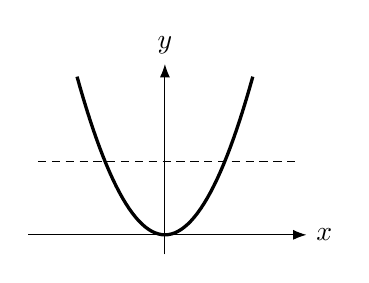
\begin{tikzpicture}[x=.62cm,y=.62cm,>=Latex]
\draw[->](-2.8,0)--(2.9,0)node[right]{$x$};
\draw[->](0,-.4)--(0,3.5)node[above]{$y$};
\draw[very thick,domain=-1.8:1.8,samples=55]plot(\x,{\x*\x});
\draw[densely dashed](-2.6,1.5)--(2.7,1.5);
\end{tikzpicture}
\par\footnotesize Neprostá: vodorovná přímka protíná dvakrát
\end{minipage}
\end{center}

\blok{Geometrický obraz inverzní funkce}
Při obrácení funkčního přiřazení si \textbf{body vymění souřadnice}. Bod $A=[a;b]$ na původním grafu se změní na bod $A'=[b;a]$. Geometricky jde o zrcadlení podle přímky $\boldsymbol{y=x}$.

\begin{definiceBox}[title={Definice - Inverzní funkce}]
K prosté funkci $f$ existuje \textbf{inverzní funkce} $f^{-1}$, která každé dosažené funkční hodnotě přiřadí její původní argument. Platí
\[
D(f^{-1})=H(f),\qquad H(f^{-1})=D(f).
\]
\end{definiceBox}

\begin{zadaniBox}[title={Věta - Souměrnost grafů inverzních funkcí}]
Graf funkce $f$ a graf její inverzní funkce $f^{-1}$ jsou osově souměrné podle přímky $y=x$.
\end{zadaniBox}
\poznamka{Vysvětli souměrnost fyzicky: zakresli přímku $y=x$, vyznač dvojice bodů a ukazuj jejich překlopení. Osa $y=x$ není totožná s osou $x$ ani s osou $y$.}

\begin{prikladReseniBox}[title={Příklad 2}]
Na grafu prosté funkce $f$ leží body $A=[-1;0]$, $B=[0;1]$ a $C=[1;2]$. Zakresli jejich obrazy na grafu $f^{-1}$ a oba grafy ve stejné soustavě souřadnic.
\tcblower
Odpovídající body jsou $A'=[0;-1]$, $B'=[1;0]$ a $C'=[2;1]$. Původní body leží na přímce $f$; odražené body leží na její inverzní přímce. Grafy jsou souměrné podle $y=x$.
\end{prikladReseniBox}

\begin{center}
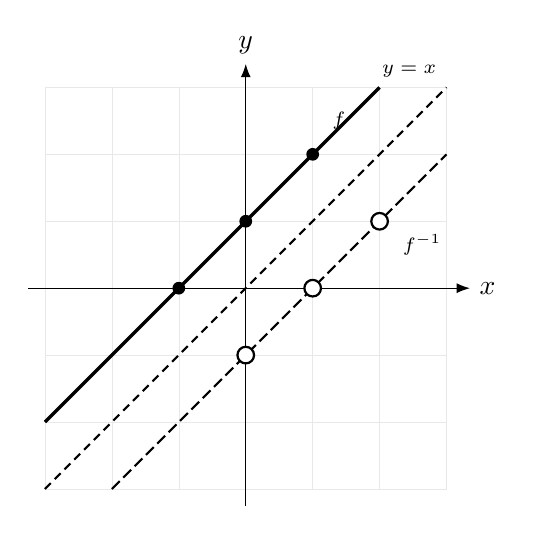
\begin{tikzpicture}[x=.85cm,y=.85cm,>=Latex]
\draw[step=1,gray!18,very thin](-3,-3)grid(3,3);
\draw[->](-3.25,0)--(3.35,0)node[right]{$x$};
\draw[->](0,-3.25)--(0,3.35)node[above]{$y$};
\draw[densely dashed,thick](-3,-3)--(3,3)node[above left,font=\scriptsize]{$y=x$};
\draw[very thick](-3,-2)--(2,3);
\draw[thick,dash pattern=on 4pt off 1.8pt](-2,-3)--(3,2);
\fill (-1,0)circle(2.3pt) (0,1)circle(2.3pt) (1,2)circle(2.3pt);
\draw[fill=white,thick](0,-1)circle(3pt) (1,0)circle(3pt) (2,1)circle(3pt);
\node[font=\scriptsize,anchor=west]at(1.15,2.5){$f$};
\node[font=\scriptsize,anchor=west]at(2.2,.65){$f^{-1}$};
\end{tikzpicture}
\end{center}
\poznamka{Plné body představují původní funkci, prázdné jejich obrazy. Obě osy jsou ve stejném měřítku, aby osová souměrnost byla skutečně vidět.}

\begin{prikladReseniBox}[title={Příklad 3}]
Parabola $y=x^2$ není na $\mathbb R$ prostá. Ponech v obrázku pouze větev pro $x\ge0$ a graficky sestroj její inverzi. Jak se změní definiční obor a obor hodnot?
\tcblower
Pravá větev obsahuje například body $[0;0]$, $[1;1]$, $[2;4]$. Po zrcadlení podle $y=x$ získáme body $[0;0]$, $[1;1]$, $[4;2]$. Obě funkce mají definiční obor i obor hodnot $\langle0;+\infty)$. Inverzní graf je obrazem pravé větve paraboly.
\end{prikladReseniBox}

\begin{center}
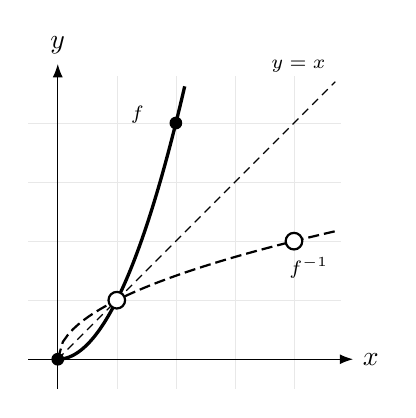
\begin{tikzpicture}[x=.75cm,y=.75cm,>=Latex]
\draw[step=1,gray!18,very thin](-.5,-.5)grid(4.8,4.8);
\draw[->](-.5,0)--(5.0,0)node[right]{$x$};
\draw[->](0,-.5)--(0,5.0)node[above]{$y$};
\draw[densely dashed](0,0)--(4.7,4.7)node[above left,font=\scriptsize]{$y=x$};
\draw[very thick,domain=0:2.15,samples=55]plot(\x,{\x*\x});
\draw[thick,dash pattern=on 4pt off 1.8pt,domain=0:4.7,samples=55]plot(\x,{sqrt(\x)});
\fill (0,0)circle(2.3pt) (1,1)circle(2.3pt) (2,4)circle(2.3pt);
\draw[fill=white,thick](1,1)circle(3pt) (4,2)circle(3pt);
\node[font=\scriptsize]at(1.35,4.15){$f$};
\node[font=\scriptsize]at(4.25,1.55){$f^{-1}$};
\end{tikzpicture}
\end{center}

\clearpage
\blok{Samostatná práce}
\begin{zadaniReseniBox}[title={Samostatná práce 1}]
\begin{enumerate}[label=\alph*)]
\item Zrcadli podle $y=x$ body $P=[-2;1]$, $Q=[0;3]$ a $R=[2;5]$.
\item Uvažuj graf úsečky z $[-2;-1]$ do $[1;2]$. Urči koncové body grafu inverze a sestroj ho.
\item Rozhodni pomocí vodorovného testu, zda má $y=|x|$ na $\mathbb R$ inverzní funkci.
\end{enumerate}
\tcblower
\begin{enumerate}[label=\alph*)]
\item $P'=[1;-2]$, $Q'=[3;0]$, $R'=[5;2]$.
\item Inverzní úsečka má koncové body $[-1;-2]$ a $[2;1]$; obě jsou souměrné podle $y=x$.
\item Nemá: například vodorovná přímka $y=2$ původní graf protne v bodech s argumenty $-2$ a $2$.
\end{enumerate}
\end{zadaniReseniBox}

\begin{zadaniReseniBox}[title={Rozšíření 1}]
Mohou graf prosté funkce a graf její inverze mít společné body mimo $y=x$? Uveď grafický příklad.
\tcblower
Ano. Například graf $f(x)=-x$ je souměrný sám se sebou podle přímky $y=x$; graf $f$ a $f^{-1}$ splývá a obsahuje body mimo osu souměrnosti.
\end{zadaniReseniBox}

\begin{zadaniReseniBox}[title={Domácí úkol}]
\begin{enumerate}[label=\alph*)]
\item Na grafu prosté funkce jsou body $[-3;1]$, $[-1;2]$, $[1;4]$. Napiš jejich obrazy po zrcadlení podle $y=x$.
\item Nakresli graf $f(x)=x+2$ a graf jeho inverze pouze geometricky pomocí osy $y=x$.
\item Vysvětli, proč se celá parabola $y=x^2$ při zrcadlení podle $y=x$ nezmění v graf funkce.
\item Graf funkce $f$ prochází body $[0;3]$ a $[2;5]$. Jakými body prochází její grafická inverze?
\item Nakresli graf $f(x)=2x-4$ a zrcadlený graf podle $y=x$ bez výpočtu předpisu.
\end{enumerate}
\tcblower
\begin{enumerate}[label=\alph*)]
\item $[1;-3]$, $[2;-1]$, $[4;1]$.
\item Přímka původní funkce prochází body $[-2;0]$ a $[0;2]$; inverzní graf prochází body $[0;-2]$ a $[2;0]$.
\item Vodorovná přímka protíná původní parabolu někdy dvakrát, a tedy po zrcadlení bude odpovídat dvěma různým výstupům při stejném argumentu.
\item $[3;0]$ a $[5;2]$.
\item Např. body $[0;-4]$, $[2;0]$ se změní na $[-4;0]$, $[0;2]$.
\end{enumerate}
\end{zadaniReseniBox}
\end{document}
